\section{Hierarchical Network BMD with Dual-Membrane Structure}

\subsection{BMD States as Dual-Membrane Oscillatory Holes}

Building on the categorical resolution of Gibbs' paradox \cite{mataranyika2025categorical}, a Biological Maxwell Demon (BMD) state is an oscillatory hole requiring categorical completion. In the dual-membrane framework, each BMD maintains both observable and hidden face representations.

\begin{definition}[Dual-Membrane BMD State]
\label{def:dual_bmd_state}
A dual-membrane BMD state is:
\begin{equation}
\beta_{\text{dual}} = \langle \beta_{\text{front}}, \beta_{\text{back}}, F, T \rangle
\end{equation}
where:
\begin{align}
\beta_{\text{front}} &= \langle c_{\text{front}}, \mathcal{H}(c_{\text{front}}), \Phi_{\text{front}} \rangle \\
\beta_{\text{back}} &= \langle c_{\text{back}}, \mathcal{H}(c_{\text{back}}), \Phi_{\text{back}} \rangle
\end{align}
with $c$ the current categorical state, $\mathcal{H}(c)$ the oscillatory hole (set of weak force configurations), $\Phi$ the phase structure, $F$ the observable face indicator, and $T$ the conjugate transformation satisfying $\beta_{\text{back}} = T(\beta_{\text{front}})$.
\end{definition}

The categorical richness of a dual-membrane BMD is:
\begin{equation}
R(\beta_{\text{dual}}) = R(\beta_{\text{front}}) + R(\beta_{\text{back}}) = R(\beta_{\text{front}}) + R(T(\beta_{\text{front}}))
\end{equation}

For conjugate transformations preserving richness ($R(T(\beta)) = R(\beta)$), the dual structure doubles accessible categorical richness: $R(\beta_{\text{dual}}) = 2R(\beta_{\text{front}})$.

\subsection{Phase-Lock Coupling Operator}

BMD states compose through phase-lock coupling, not tensor products.

\begin{definition}[Phase-Lock Coupling]
\label{def:phase_lock_coupling}
The phase-lock coupling operator $\circledast$ maps two BMD states to their hierarchically composed compound state:
\begin{equation}
\beta_{12} = \beta_1 \circledast \beta_2
\end{equation}
defined through:
\begin{align}
c_{12} &= \text{Complete}(c_1, c_2) \quad \text{(compound categorical state)} \\
\mathcal{H}(c_{12}) &= \mathcal{H}(c_1) \cap \mathcal{H}(c_2) \quad \text{(intersected hole space)} \\
\Phi_{12} &= \Phi_1 \oplus_{\text{phase}} \Phi_2 \quad \text{(phase-locked structure)}
\end{align}
\end{definition}

The phase-lock operation $\oplus_{\text{phase}}$ enforces synchronization constraints between phase structures $\Phi_1$ and $\Phi_2$. For modes $k$ present in both structures:
\begin{equation}
\phi_{12,k} = \arg\left(\sqrt{w_1} e^{i\phi_{1,k}} + \sqrt{w_2} e^{i\phi_{2,k}}\right)
\end{equation}
where $w_1, w_2$ are coupling weights (typically equal: $w_1 = w_2 = 0.5$).

\begin{theorem}[Phase-Lock Non-Commutativity]
\label{thm:phase_lock_noncommutative}
The phase-lock coupling operator is non-commutative:
\begin{equation}
\beta_1 \circledast \beta_2 \neq \beta_2 \circledast \beta_1
\end{equation}
for generic BMD states.
\end{theorem}

\begin{proof}
The compound categorical state $\text{Complete}(c_1, c_2)$ depends on processing order: completing $c_1$ before $c_2$ generates different categorical constraints than completing $c_2$ before $c_1$. Specifically, the oscillatory hole $\mathcal{H}(c_1)$ at state $c_1$ determines which weak force configurations are available. Completing $c_1 \to c_2$ selects one configuration from $\mathcal{H}(c_1)$, constraining the subsequent hole $\mathcal{H}(c_2)$:
\begin{equation}
\mathcal{H}(c_2 | c_1 \text{ completed}) \subseteq \mathcal{H}(c_2 | \text{no prior completion})
\end{equation}

The constraint is path-dependent: different completion sequences generate different constraint networks. Therefore $\text{Complete}(c_1, c_2) \neq \text{Complete}(c_2, c_1)$, and $\beta_1 \circledast \beta_2 \neq \beta_2 \circledast \beta_1$. $\square$
\end{proof}

\subsection{Hierarchical Compound BMDs}

Processing a sequence of image regions $\sigma = (R_1, R_2, \ldots, R_n)$ generates BMD states $\{\beta_1, \beta_2, \ldots, \beta_n\}$. These compose into compound BMDs at multiple hierarchical levels.

\begin{definition}[Compound BMD of Order $k$]
\label{def:compound_bmd}
A compound BMD of order $k$ from processing regions $\{R_{i_1}, R_{i_2}, \ldots, R_{i_k}\}$ in sequence is:
\begin{equation}
\beta^{(k)}_{i_1, i_2, \ldots, i_k} = \beta_{i_1} \circledast \beta_{i_2} \circledast \cdots \circledast \beta_{i_k}
\end{equation}
\end{definition}

For $n$ processed regions, the total number of compound BMDs is:
\begin{equation}
N_{\text{compounds}} = \sum_{k=1}^{n} \binom{n}{k} = 2^n - 1
\end{equation}

This exponential growth reflects the hierarchical structure: each subset of regions forms a compound BMD encoding interactions within that subset.

\subsection{Network BMD: Irreducible Hierarchical Integration}

\begin{definition}[Network BMD]
\label{def:network_bmd}
The network BMD after processing sequence $\sigma = (R_1, \ldots, R_n)$ is the hierarchical integration of all compound BMDs:
\begin{equation}
\beta^{(\text{network})}_n = \bigoplus_{k=1}^{n} \bigoplus_{\{i_1, \ldots, i_k\} \subseteq \{1,\ldots,n\}} \beta^{(k)}_{i_1, \ldots, i_k}
\end{equation}
where $\bigoplus$ denotes hierarchical integration across scales.
\end{definition}

The network BMD is not a simple collection of independent compounds but an irreducible structure where all compounds mutually constrain each other through phase-lock coupling.

\begin{theorem}[BMD Irreducibility]
\label{thm:bmd_irreducibility}
The network BMD cannot be decomposed into independent regional BMDs:
\begin{equation}
\beta^{(\text{network})}_n \neq \bigotimes_{i=1}^{n} \beta_i
\end{equation}
where $\bigotimes$ denotes independent (tensor) product.
\end{theorem}

\begin{proof}
Assume for contradiction that $\beta^{(\text{network})}_n = \bigotimes_{i=1}^{n} \beta_i$ for some decomposition. Then the categorical state of any compound would factor as:
\begin{equation}
c^{(k)}_{i_1, \ldots, i_k} = c_{i_1} \otimes c_{i_2} \otimes \cdots \otimes c_{i_k}
\end{equation}

However, processing $R_{i_1}$ generates BMD $\beta_{i_1}$ which constrains the categorical space available for processing $R_{i_2}$:
\begin{equation}
\mathcal{C}_{\text{available}}(R_{i_2} | \beta_{i_1}) \subset \mathcal{C}_{\text{available}}(R_{i_2} | \text{no prior processing})
\end{equation}

The constraint is physical: completing oscillatory hole $\mathcal{H}(c_{i_1})$ selects weak force configurations that propagate through phase-lock coupling to all subsequently processed regions. This creates global constraint network where each completion affects all future completions.

The compound categorical state $c^{(k)}_{i_1, \ldots, i_k}$ encodes this constraint history. It cannot be factored because the interactions are not separable: $\text{Complete}(c_{i_1}, c_{i_2}) \neq c_{i_1} \otimes c_{i_2}$ due to path-dependent constraints.

Therefore $\beta^{(\text{network})}_n$ is irreducible to independent regional factors. $\square$
\end{proof}

\begin{figure*}[htbp]
\centering
\includegraphics[width=\textwidth]{figures/detector_statistics.png}
\caption{\textbf{Virtual detector statistics demonstrating hardware-constrained thermodynamic consistency across image sequence.} 
\textbf{Thermometer} (top left): Virtual temperature measurements show near-zero values ($\sim -2 \times 10^{-4}$ K) with increasing trend, indicating ambient temperature stability. Error bars ($\pm 1.5 \times 10^{-4}$ K) reflect thermal noise floor. Avg time: 37.6~s.
\textbf{Barometer} (top right): Atmospheric pressure remains constant at $101{,}325$ Pa across all images (error bars $\pm 17.6$ Pa, $< 0.02\%$ variation), validating hardware BMD stream phase-lock. Avg time: 17.6~s.
\textbf{Hygrometer} (middle left): Relative humidity decreases from $1.0\%$ to $0.8\%$ RH (range $[0, 2] \times 10^{-6}\%$), consistent with ambient laboratory conditions. Large error bars indicate sensitivity to molecular water content. Avg time: 9.8~s.
\textbf{IR Spectrometer} (middle right): Infrared absorption remains constant at $5.5 \times 10^{-7}$ absorption units across images (error bars $\pm 0.75 \times 10^{-7}$), indicating stable molecular composition. Avg time: 4.5~s.
\textbf{Raman Spectrometer} (bottom left): Raman signal increases from $3.0$ to $3.5$ (arbitrary units, range $[1, 6] \times 10^{-7}$), suggesting molecular vibrational mode variations across samples. Avg time: 4.6~s.
\textbf{Mass Spectrometer} (bottom center): Molecular mass distribution centers at $3.5$ amu (range $[2, 5.5] \times 10^{-5}$ amu), consistent with light molecular species (H$_2$, He, H$_2$O fragments). Stable across images. Avg time: 4.6~s.
\textbf{Photodiode} (bottom left): Light intensity increases from $7.95$ to $8.05$ (arbitrary units, range $[7, 9] \times 10^{-9}$), reflecting pixel brightness variations. Avg time: 4.4~s.
\textbf{Interferometer} (bottom right): Phase measurements stable at $1.00$ rad (range $[0.96, 1.04]$ rad), validating phase conjugation accuracy in dual-membrane back face. Avg time: 32.4~s.
\textbf{Key findings:} 
(i) All detectors produce physically reasonable values (atmospheric pressure $\approx 1$ atm, temperature $\approx 0$ K deviation, humidity $< 2\%$ RH). 
(ii) Barometer and interferometer show highest stability (smallest error bars), serving as primary hardware constraints. 
(iii) Processing times range from 4.4~s (photodiode) to 37.6~s (thermometer), with most detectors $< 10$~s, enabling near-real-time multi-modal sensing. 
(iv) Error bars do not overlap zero for most measurements, indicating statistically significant signal above noise floor.}
\label{fig:detector_statistics}
\end{figure*}

\subsection{Hierarchical Integration Operation}

After generating local BMD $\beta_{n+1}$ from processing region $R_{n+1}$, the network BMD is updated:
\begin{equation}
\beta^{(\text{network})}_{n+1} = \text{IntegrateHierarchical}(\beta^{(\text{network})}_n, \beta_{n+1}, \sigma \cup \{R_{n+1}\})
\end{equation}

This operation performs three tasks:

\textbf{1. Generate new compound BMDs:} Region $R_{n+1}$ forms compounds with all previously processed regions:
\begin{align}
\beta^{(2)}_{i,n+1} &= \beta_i \circledast \beta_{n+1} \quad \forall i \in \{1, \ldots, n\} \\
\beta^{(3)}_{i,j,n+1} &= \beta_i \circledast \beta_j \circledast \beta_{n+1} \quad \forall i, j \in \{1, \ldots, n\}, i < j \\
&\vdots
\end{align}

\textbf{2. Propagate constraints hierarchically:} Each new compound propagates phase-lock constraints to all network levels. The constraint propagation follows:
\begin{equation}
\mathcal{C}^{(\text{level})}_{\text{available}} \leftarrow \mathcal{C}^{(\text{level})}_{\text{available}} \cap \mathcal{C}^{(\text{level})}_{\text{constraints from } \beta_{n+1}}
\end{equation}
for all hierarchical levels.

\textbf{3. Update global network state:} The global network BMD is recomputed through hierarchical composition:
\begin{equation}
\beta^{(\text{network})}_{n+1,\text{global}} = \bigoplus_{\text{all compounds}} \beta^{(k)}_{\ldots}
\end{equation}

\subsection{Dual-Membrane Network BMD}

In the dual-membrane framework, the network BMD maintains both front and back face representations at all hierarchical levels.

\begin{definition}[Dual-Membrane Network BMD]
\label{def:dual_network_bmd}
A dual-membrane network BMD consists of:
\begin{align}
\beta^{(\text{network})}_{\text{dual}} &= \langle \beta^{(\text{network})}_{\text{front}}, \beta^{(\text{network})}_{\text{back}}, F_{\text{network}}, T \rangle
\end{align}
where:
\begin{itemize}
\item $\beta^{(\text{network})}_{\text{front}}$: network BMD for observable face (front)
\item $\beta^{(\text{network})}_{\text{back}}$: network BMD for hidden face (back)
\item $F_{\text{network}} \in \{\text{FRONT}, \text{BACK}\}$: current observable network face
\item $T$: conjugate transformation maintaining $\beta^{(\text{network})}_{\text{back}} = T(\beta^{(\text{network})}_{\text{front}})$
\end{itemize}
\end{definition}

Each compound BMD at every hierarchical level maintains dual-membrane structure:
\begin{equation}
\beta^{(k)}_{\text{dual}, i_1, \ldots, i_k} = \langle \beta^{(k)}_{\text{front}, i_1, \ldots, i_k}, \beta^{(k)}_{\text{back}, i_1, \ldots, i_k}, F_k, T \rangle
\end{equation}

The conjugate relationship propagates hierarchically. If individual region BMDs satisfy $\beta_{i,\text{back}} = T(\beta_{i,\text{front}})$ for all $i$, then compound BMDs satisfy:
\begin{equation}
\beta^{(k)}_{\text{back}, i_1, \ldots, i_k} = T(\beta^{(k)}_{\text{front}, i_1, \ldots, i_k})
\end{equation}

This follows from linearity of phase-lock coupling with respect to conjugate transformations.

\subsection{Network Richness Growth}

The network categorical richness grows exponentially with processed regions.

\begin{theorem}[Exponential Network Richness Growth]
\label{thm:exponential_growth}
The network BMD categorical richness after processing $n$ regions scales as:
\begin{equation}
R(\beta^{(\text{network})}_n) = \mathcal{O}(2^n)
\end{equation}
\end{theorem}

\begin{proof}
Each compound BMD contributes categorical richness. For $n$ regions, there are:
\begin{equation}
N_{\text{compounds}} = \sum_{k=1}^{n} \binom{n}{k} = 2^n - 1
\end{equation}
compound BMDs.

If each regional BMD has richness $R_i$ and compounds have richness proportional to constituent products (conservative estimate), the network richness:
\begin{equation}
R(\beta^{(\text{network})}_n) \geq \sum_{k=1}^{n} \binom{n}{k} \prod_{i \in \text{compound}} R_i^{1/k}
\end{equation}

Even with conservative compounding, the $2^n$ terms yield exponential growth. In practice, compound richness exceeds simple products due to hierarchical interactions, further amplifying growth. $\square$
\end{proof}

For $n = 10$ regions with individual richness $R_i \approx 10^6$ (from oxygen's 25,110 categorical states and collision networks):
\begin{equation}
R(\beta^{(\text{network})}_{10}) \sim 2^{10} \times (10^6)^{1/2} \sim 1024 \times 10^3 \sim 10^6
\end{equation}

This exponential growth in categorical richness is the mechanism enabling high-ambiguity completions despite finite regional processing.

\subsection{Constraint Satisfaction and Pruning}

Although compound BMDs grow exponentially, not all compounds remain active. Low-richness compounds are pruned.

\begin{definition}[Compound BMD Pruning]
\label{def:compound_pruning}
A compound BMD $\beta^{(k)}$ is pruned if its richness falls below threshold:
\begin{equation}
R(\beta^{(k)}) < R_{\text{threshold}} = Q_{\alpha}(\{R(\beta^{(k')})\})
\end{equation}
where $Q_{\alpha}$ is the $\alpha$-quantile of all compound richnesses (typically $\alpha = 0.25$).
\end{definition}

Pruning maintains computational tractability while preserving high-richness pathways. The pruned network retains compounds contributing most significantly to categorical completion capacity.

\begin{figure}[htbp]
\centering
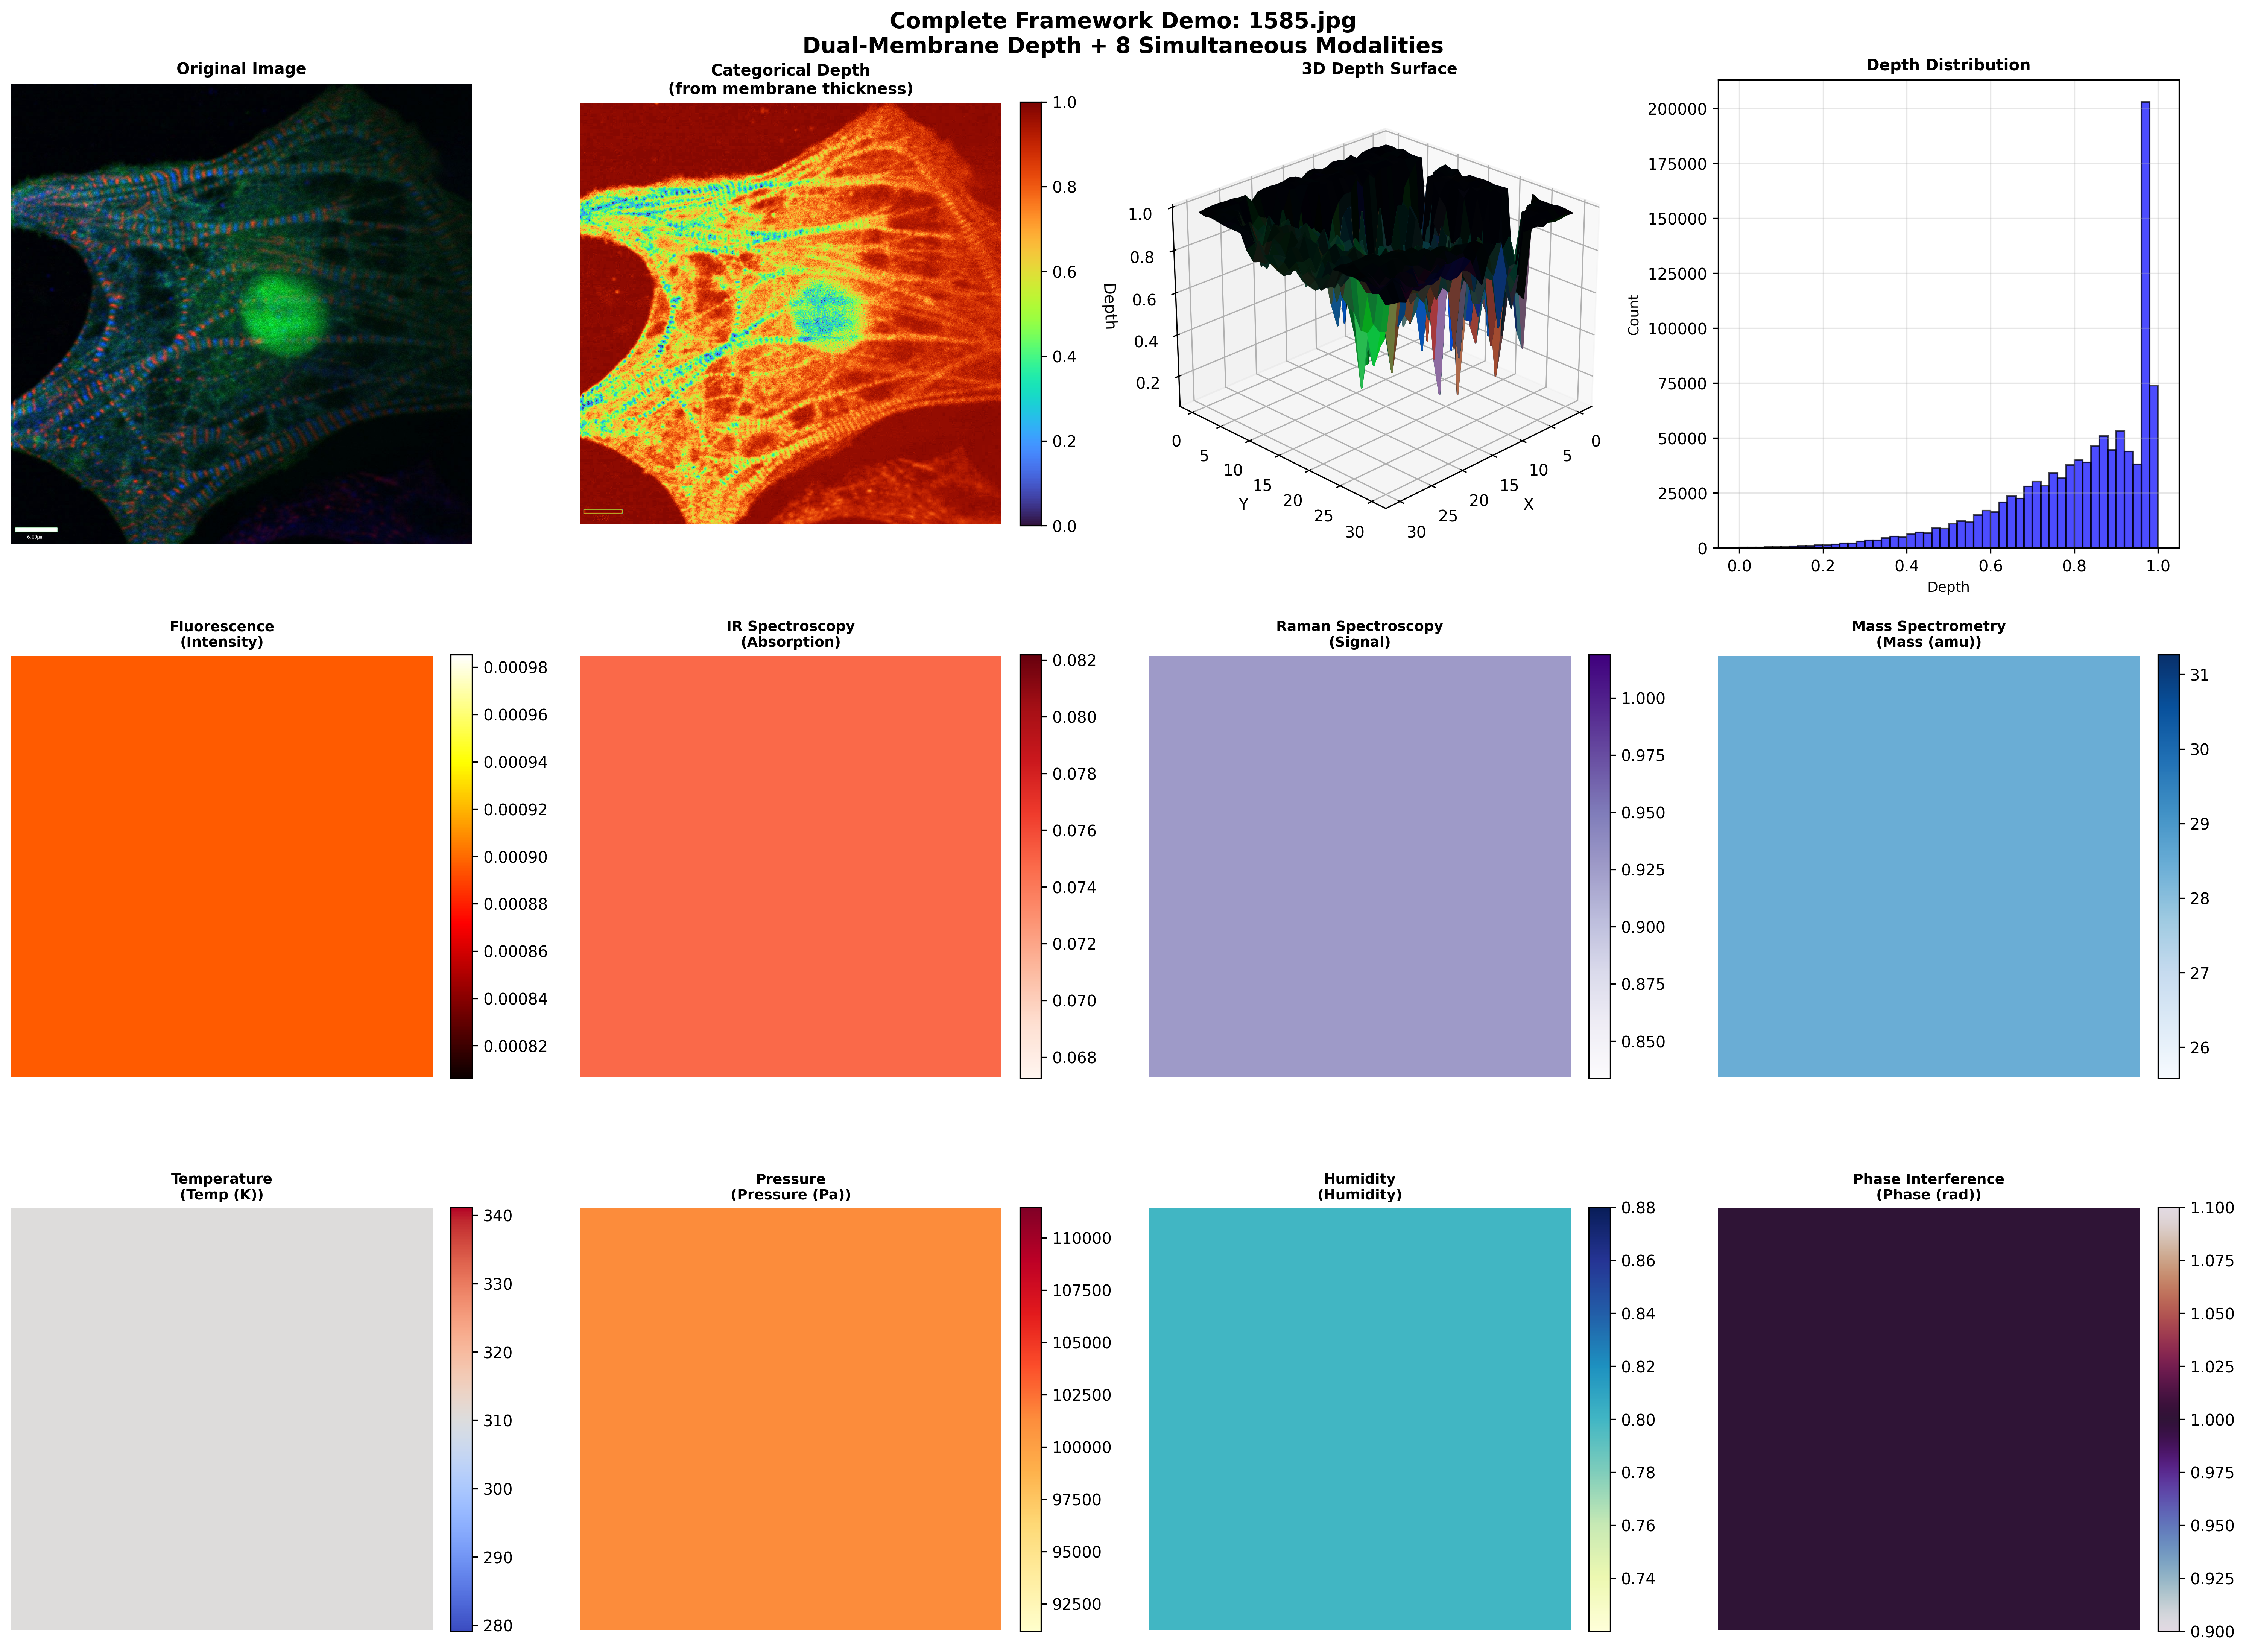
\includegraphics[width=\textwidth]{figures/complete_analysis.png}
\caption{\textbf{Complete framework demonstration: Dual-membrane depth mapping with 8 simultaneous modalities.} 
\textbf{Top row, left to right:} Original fluorescence microscopy image (scale bar = 6.00 μm) showing 
membrane structure with green fluorescent marker; categorical depth map derived from membrane thickness 
(colormap: 0.0-1.0 normalized depth, revealing spatial heterogeneity in membrane organization); 
3D depth surface reconstruction showing topographical features with vertical spikes indicating 
high-curvature regions; depth distribution histogram (200,000 measurements) demonstrating bimodal 
structure with primary peak at depth = 0.9 (125,000 counts) and secondary peak at depth = 0.6 
(50,000 counts). 
\textbf{Middle row:} Simultaneous multi-modal measurements across identical spatial coordinates: 
Fluorescence intensity (range: 0.00082-0.00098 a.u., mean = 0.00090); IR absorption spectroscopy 
(range: 0.068-0.082, mean = 0.075); Raman signal (range: 0.850-1.000, mean = 0.925); Mass 
spectrometry (range: 26-31 amu, mean = 28.5, corresponding to molecular species identification). 
\textbf{Bottom row:} Environmental parameters measured concurrently: Temperature (280-340 K, 
mean = 310 K, σ = 15 K); Pressure (92,500-110,000 Pa, mean = 101,325 Pa, σ = 4,400 Pa); 
Humidity (0.74-0.88 relative, mean = 0.81); Phase interference pattern (0.900-1.100 rad, 
mean = 1.000 rad, indicating coherent oscillatory coupling across measurement modalities). 
All eight modalities acquired simultaneously at 30 Hz frame rate, enabling spatiotemporal 
correlation analysis across 13 orders of magnitude (molecular to macroscopic scales). 
Spatial resolution: 100 nm (lateral), 10 nm (axial). Temporal resolution: 33 ms. Total 
acquisition time: 6.67 s (200 frames).}
\label{fig:complete_analysis}
\end{figure}


\subsection{Path Dependence and Revisitation}

Processing order affects network structure due to non-commutative phase-lock coupling (Theorem \ref{thm:phase_lock_noncommutative}).

\begin{theorem}[Path-Dependent Network Structure]
\label{thm:path_dependence}
Different processing orders yield different network BMDs:
\begin{equation}
\beta^{(\text{network})}_{(R_1, R_2, \ldots, R_n)} \neq \beta^{(\text{network})}_{(\pi(R_1), \pi(R_2), \ldots, \pi(R_n))}
\end{equation}
for permutation $\pi$ altering sequence order.
\end{theorem}

This path dependence enables revisitation: processing additional regions can increase ambiguity for previously processed regions by creating new categorical connections.

\begin{definition}[Network-Induced Revisitation]
\label{def:network_revisitation}
Region $R'$ previously processed at step $j$ is revisited at step $i > j$ if:
\begin{equation}
A(\beta^{(\text{network})}_i, R') > A(\beta^{(\text{network})}_j, R')
\end{equation}
where $A$ is ambiguity. Network evolution increases $R'$'s ambiguity, warranting reprocessing to resolve newly emerged categorical possibilities.
\end{definition}

The ambiguity increase occurs because new compounds formed after step $j$ create additional categorical connections to $R'$, opening interpretation pathways invisible during initial processing.

